\documentclass[12pt]{article}
\usepackage[utf8]{inputenc}
\usepackage[T1]{fontenc}
\usepackage{graphicx,amsmath,amsfonts,amssymb,float,caption,geometry,hyperref,url,booktabs,listings,xcolor}
\geometry{a4paper,margin=2.5cm}
\graphicspath{{figures/}}
\lstset{basicstyle=\ttfamily\scriptsize,breaklines=true,numbers=left,numberstyle=\tiny,frame=single,language=[90]Fortran,keywordstyle=\color{blue}}
\newcommand{\Hz}{\,\mathrm{Hz}}
\title{Sixth Assignment: Computational Neuroscience}
\author{Pierina Milla}
\date{October 2026}
\begin{document}
\maketitle

\noindent\textbf{Methods.} All programs are written in Fortran~90 (Appendix) and use units of ms, mV, pA, pF, M$\Omega$ and nS, for which $1\,\mathrm{pA/pF}=1\,\mathrm{mV/ms}$ and $1\,\mathrm{nS\cdot mV}=1\,\mathrm{pA}$. The deterministic runs use the Euler method and the noisy runs the Euler--Maruyama method, with $\Delta t=0.01$ ms and $t_{\max}=2$ s unless stated otherwise. Spike times are obtained by linear interpolation, $t^*=t_{k-1}+\Delta t\,(V_L-V_{k-1})/(V_k-V_{k-1})$, and the absolute refractory period holds $V=V_{\rm redef}$ until $t^*+\tau_{\rm ref}$. Firing rates are $f=N_{\rm spikes}/t_{\max}$ (resolution $0.5\Hz$). Every noisy run uses a different random seed.

%=====================================================================
\section{Question 1: Leaky integrate-and-fire neuron}
The model is $C\dot V=(V_{\rm rep}-V)/R+I$ with $V_{\rm rep}=-70$ mV, $R=40$ M$\Omega$, $C=250$ pF, $V_L=-50$ mV, $V_{\rm redef}=-65$ mV, $\tau_{\rm ref}=2$ ms. The membrane time constant is $\tau_m=RC=10$ ms.

\subsection{(a) $f$--$I$ curve}
\paragraph{Analytical result.} For constant $I$ the solution is $V(t)=V_\infty+(V_{\rm redef}-V_\infty)e^{-t/\tau_m}$ with $V_\infty=V_{\rm rep}+RI$. The threshold is reached only if $V_\infty>V_L$, i.e.\ $I>I_L=(V_L-V_{\rm rep})/R=500$ pA. The time to go from $V_{\rm redef}$ to $V_L$ is $\tau_m\ln\frac{RI-(V_{\rm redef}-V_{\rm rep})}{RI-(V_L-V_{\rm rep})}$, so
\begin{equation}
f(I)=\left[\tau_{\rm ref}+\tau_m\ln\frac{RI-(V_{\rm redef}-V_{\rm rep})}{RI-(V_L-V_{\rm rep})}\right]^{-1}\ (I>I_L),\qquad f=0\ (I\le I_L).
\end{equation}
Setting $f=150$ Hz gives $RI=62.0$ mV, i.e.\ $I\approx1551$ pA, so the sweep covers $400\le I\le1600$ pA in steps of $10$ pA.
\begin{figure}[H]\centering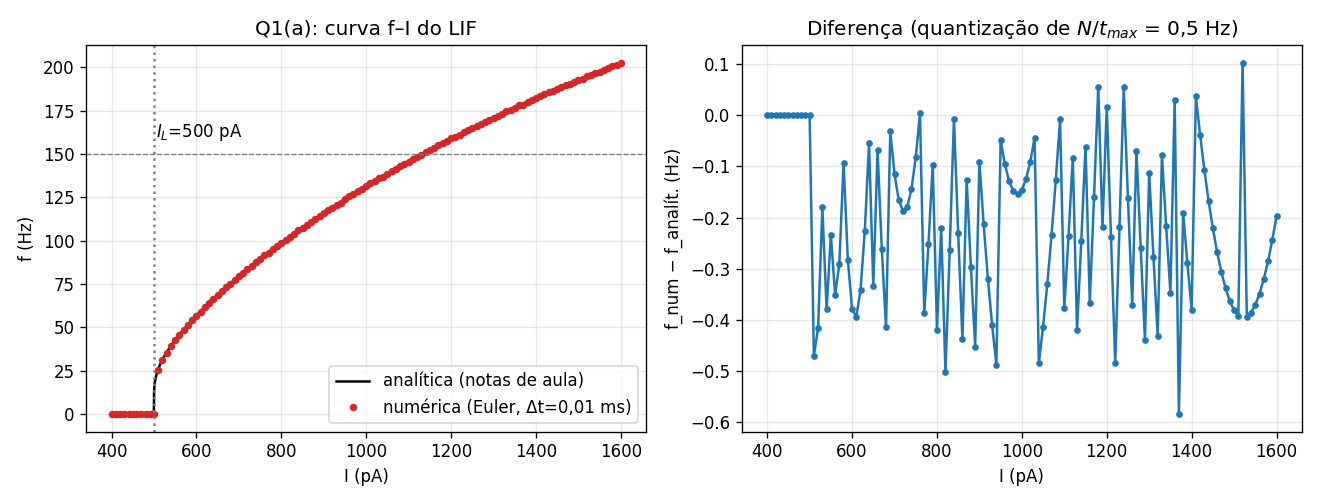
\includegraphics[width=\textwidth]{q1a_fI.png}\caption{LIF $f$--$I$ curve: numerical (symbols) and analytical (line). Right: difference.}\label{fig:q1a}\end{figure}
The numerical curve agrees with the formula to within $0.58$ Hz (maximum), which is the $0.5$ Hz quantization of $N/t_{\max}$. The curve is zero up to $I_L=500$ pA and then rises continuously from zero frequency (logarithmic divergence of the period at $I_L$), a type-I behavior.

%=====================================================================
\section{Question 2: LIF neuron with noise}
The noisy model is $\dot V=(V_{\rm rep}-V)/\tau_m+I/C+\sigma w(t)$, integrated with $V_{n+1}=V_n+f(V_n)\Delta t+\sigma\tilde w_n\sqrt{\Delta t}$, $\tilde w_n\sim\mathcal N(0,1)$ (Box--Muller). For subthreshold $I$ the free membrane potential is an Ornstein--Uhlenbeck process with mean $V_\infty$ and stationary standard deviation $\sigma_V=\sigma\sqrt{\tau_m/2}$ ($=1.12$ mV for $\sigma=0.5$ and $3.35$ mV for $\sigma=1.5$).

\subsection{(a) $f$--$I$ curves with noise}
Increasing $\sigma$ from zero, the curve first departs from the $\sigma=0$ one at $\sigma_1=0.5$ mV/ms$^{1/2}$ (non-zero rates appear just below $I_L$, e.g.\ $f(450\,\mathrm{pA})=13$ Hz and $f(500\,\mathrm{pA})=29.5$ Hz versus $0$ Hz) and it changes markedly again at $\sigma_2=1.5$ mV/ms$^{1/2}$ (firing already at $400$ pA, $f=18.5$ Hz, and $f(500)=39.5$ Hz).
\begin{figure}[H]\centering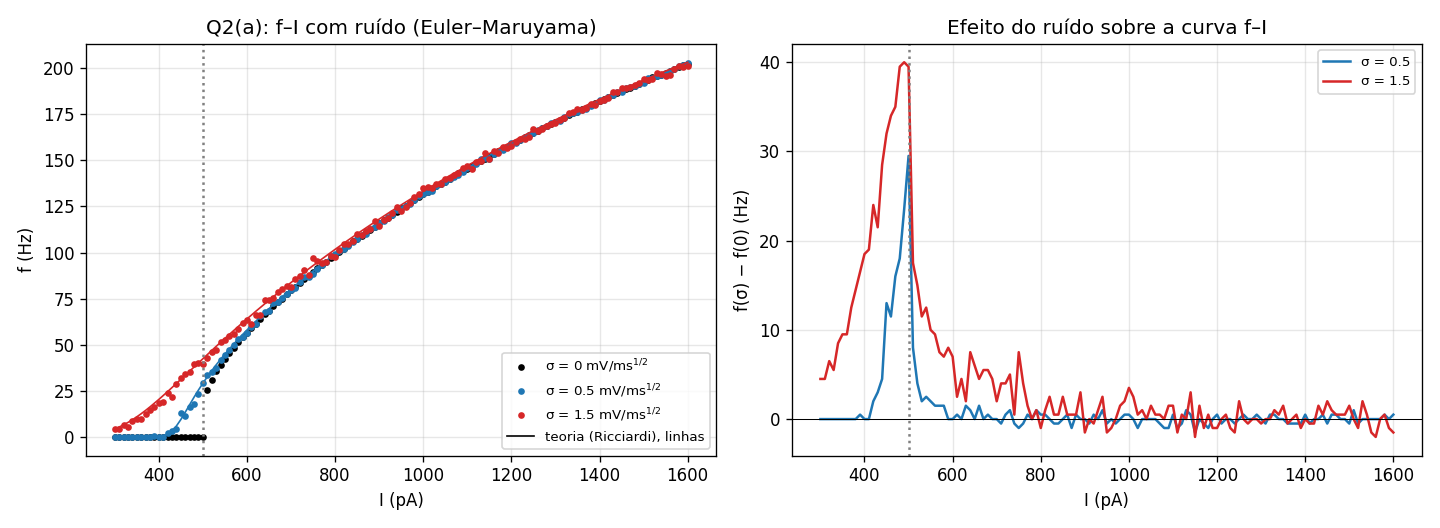
\includegraphics[width=\textwidth]{q2a_fI_ruido.png}\caption{$f$--$I$ for $\sigma=0$, $0.5$ and $1.5$ mV/ms$^{1/2}$. Lines on the left panel: Siegert--Ricciardi theory, Eq.~(\ref{eq:ric}).}\label{fig:q2a}\end{figure}
\paragraph{Interpretation.} Below $I_L$ the mean drive cannot reach threshold ($V_\infty<V_L$) but fluctuations can: spikes are noise-driven and the sharp corner of the deterministic curve at $I_L$ is smoothed into a sigmoid-like foot; the larger $\sigma$, the further below $I_L$ the firing extends and the more the threshold is blurred (maximum change $\approx30$ Hz at $I_L$ for $\sigma_1$, $\approx40$ Hz for $\sigma_2$). Far above $I_L$ the neuron is mean-driven, the interspike interval is dominated by the deterministic charging time, and the curves practically coincide (differences are within the $\pm\sqrt N/t_{\max}\approx3$--$5$ Hz sampling error of a 2-s run). The theoretical rate of the LIF with white noise (Siegert--Ricciardi) is
\begin{equation}
f^{-1}=\tau_{\rm ref}+\tau_m\sqrt\pi\int_{(V_{\rm redef}-V_\infty)/\sigma_B}^{(V_L-V_\infty)/\sigma_B}e^{u^2}\,[1+\mathrm{erf}(u)]\,du,\qquad \sigma_B=\sigma\sqrt{\tau_m},
\label{eq:ric}
\end{equation}
and reproduces the simulations (maximum difference $3.6$ and $5.3$ Hz for $\sigma_1,\sigma_2$, again of the order of the sampling error); an independent Monte Carlo first-passage calculation at $I=450$ pA, $\sigma=1.5$ gives $31.2$ Hz, in agreement with Eq.~(\ref{eq:ric}) ($31.2$ Hz) and with the simulation ($31.4$ Hz with $\Delta t=5\times10^{-4}$ ms).

\subsection{(b) Effect of $\Delta t$ on the subthreshold trajectory}
$I=300$ pA ($V_\infty=-58$ mV, below threshold), $\sigma=1.5$ mV/ms$^{1/2}$, $20$ ms. A single Brownian path is generated at the finest step ($10^{-5}$ ms) and summed to produce the increments for $\Delta t=10^{-2},10^{-3},10^{-4}$ ms, so that the trajectories are directly comparable.
\begin{figure}[H]\centering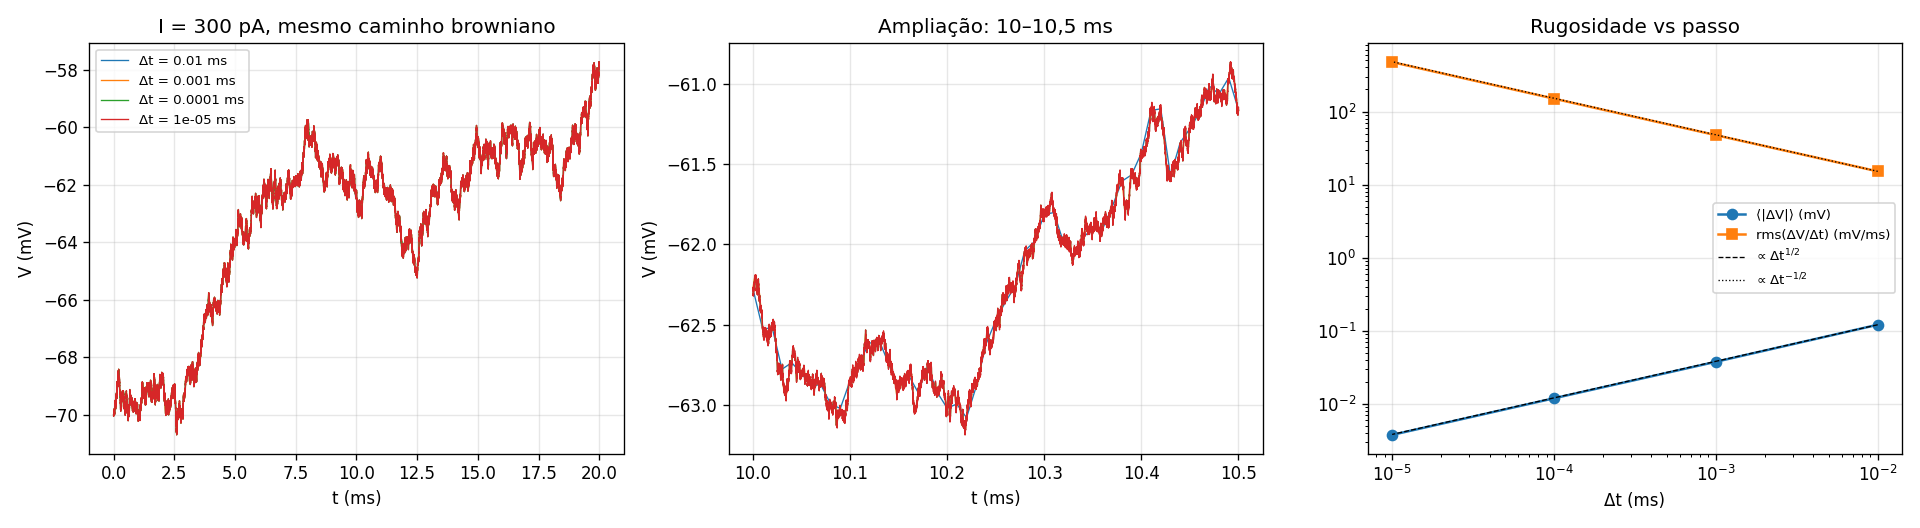
\includegraphics[width=\textwidth]{q2b_rugosidade_dt.png}\caption{Trajectories for decreasing $\Delta t$ (left), magnified (center), and roughness measures (right).}\label{fig:q2b}\end{figure}
\begin{center}\begin{tabular}{cccc}\toprule
$\Delta t$ (ms) & $\langle|\Delta V|\rangle$ (mV) & $\sum(\Delta V)^2$ (mV$^2$) & rms$(\Delta V/\Delta t)$ (mV/ms)\\\midrule
$10^{-2}$ & 0.1213 & 46.15 & 15.2\\
$10^{-3}$ & 0.0378 & 45.11 & 47.5\\
$10^{-4}$ & 0.0120 & 44.95 & 149.9\\
$10^{-5}$ & 0.0038 & 44.90 & 473.8\\\bottomrule
\end{tabular}\end{center}
\textbf{Conclusion.} The increment per step scales as $\sqrt{\Delta t}$ (it decreases by $\sqrt{10}$ for each decade), so the discrete path converges to a \emph{continuous} curve: jumps vanish as $\Delta t\to0$ and the trajectories for different $\Delta t$ overlap at the scale of the figure. However, the path does not become differentiable: the slope $\Delta V/\Delta t\propto\Delta t^{-1/2}$ diverges, and the roughness remains at every magnification (center panel). Consistently, the quadratic variation $\sum(\Delta V)^2\to\sigma^2t=45$ mV$^2$ is independent of $\Delta t$. Hence ``smooth'' means continuous, as in Brownian motion, not differentiable; this is also why $\sigma\tilde w_n\sqrt{\Delta t}$ (and not $\Delta t$) is the correct scaling of the noise term.

\subsection{(c) Regular and irregular firing}
We use $\sigma=1.5$ mV/ms$^{1/2}$ and, because the suggested values do not give a good contrast for this $\sigma$, $I_{\rm below}=400$ pA and $I_{\rm above}=800$ pA ($I_L=500$ pA). Figure~\ref{fig:q2c} shows (top) $V(t)$ with the spike mechanism turned off and the threshold (dashed) and (bottom) the same noise realization with spikes (peaks drawn by hand at $+20$ mV); the first $1000$ ms of the $2$ s run are shown.
\begin{figure}[H]\centering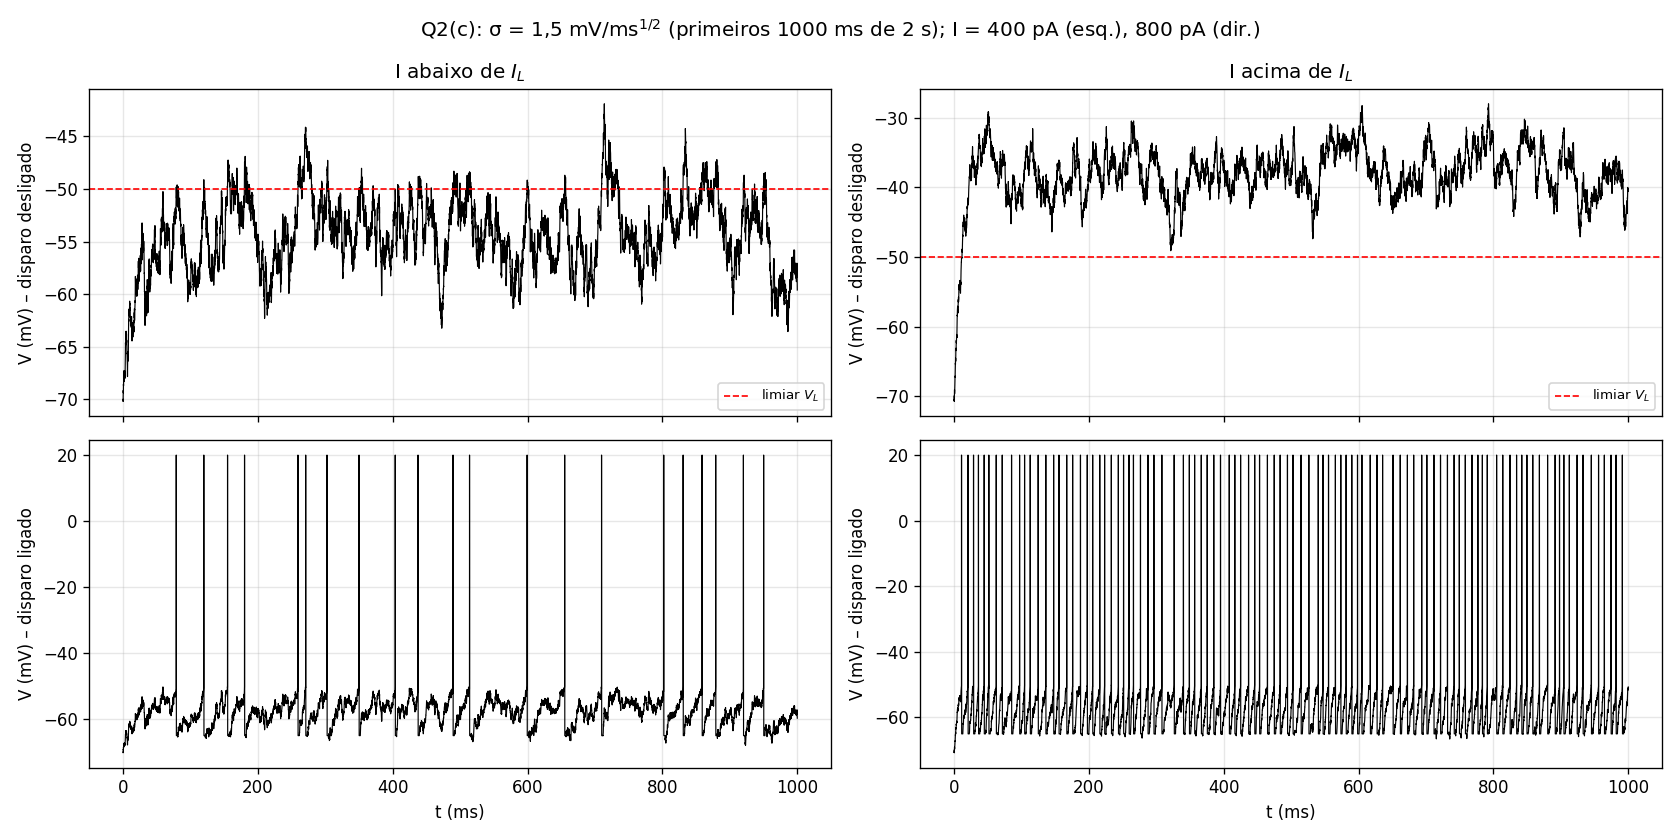
\includegraphics[width=\textwidth]{q2c_regular_irregular.png}\caption{Below threshold (left) and above threshold (right).}\label{fig:q2c}\end{figure}
\begin{center}\begin{tabular}{lccccc}\toprule
Case & $I$ (pA) & $N$ & $\langle\mathrm{ISI}\rangle$ (ms) & sd (ms) & $CV_{\rm ISI}$\\\midrule
Below & 400 & 40 & 48.56 & 27.26 & 0.56\\
Above & 800 & 203 & 9.83 & 2.67 & 0.27\\\bottomrule
\end{tabular}\end{center}
Averaged over $30$ realizations: $CV=0.67\pm0.11$ at $400$ pA and $0.23\pm0.014$ at $800$ pA; the CV decreases monotonically with $I$ (Fig.~\ref{fig:q2cb}). The firing is more irregular below threshold. There, $V_\infty<V_L$ and spikes are triggered by rare noise excursions to the threshold; the waiting times are broadly distributed (close to the exponential of a Poisson process, though $CV<1$ because of the refractory period and the reset), so the ISI distribution is wide. Above threshold the mean drive makes $V$ climb deterministically toward $V_L$ and noise only perturbs this ramp, so ISIs cluster around the deterministic charging time (plus $\tau_{\rm ref}$): firing is regular.
\begin{figure}[H]\centering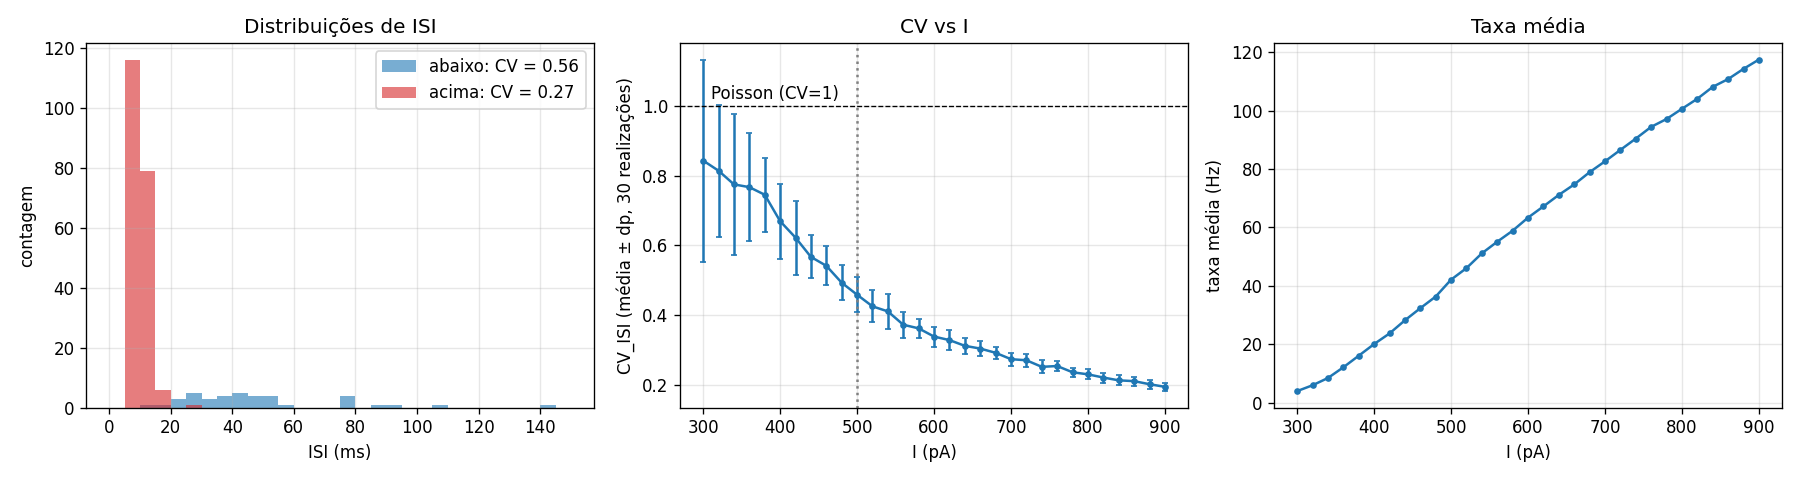
\includegraphics[width=\textwidth]{q2c_ISI_CV.png}\caption{ISI histograms, $CV_{\rm ISI}$ vs.\ $I$ and mean rate (30 seeds per current).}\label{fig:q2cb}\end{figure}

%=====================================================================
\section{Question 3: LIF with adaptation current}
The model is $C\dot V=(V_{\rm rep}-V)/R+G_a(V_{\rm redef}-V)+I$, $\dot G_a=-G_a/\tau_a$, with $V\to V_{\rm redef}$ and $G_a\to G_a+b$ at each spike; $V_{\rm redef}=-80$ mV, $b=1$ nS, $\tau_a=200$ ms, other parameters as in Question~1 (including $\tau_{\rm ref}$).

\subsection{(a) Current pulse}
\begin{figure}[H]\centering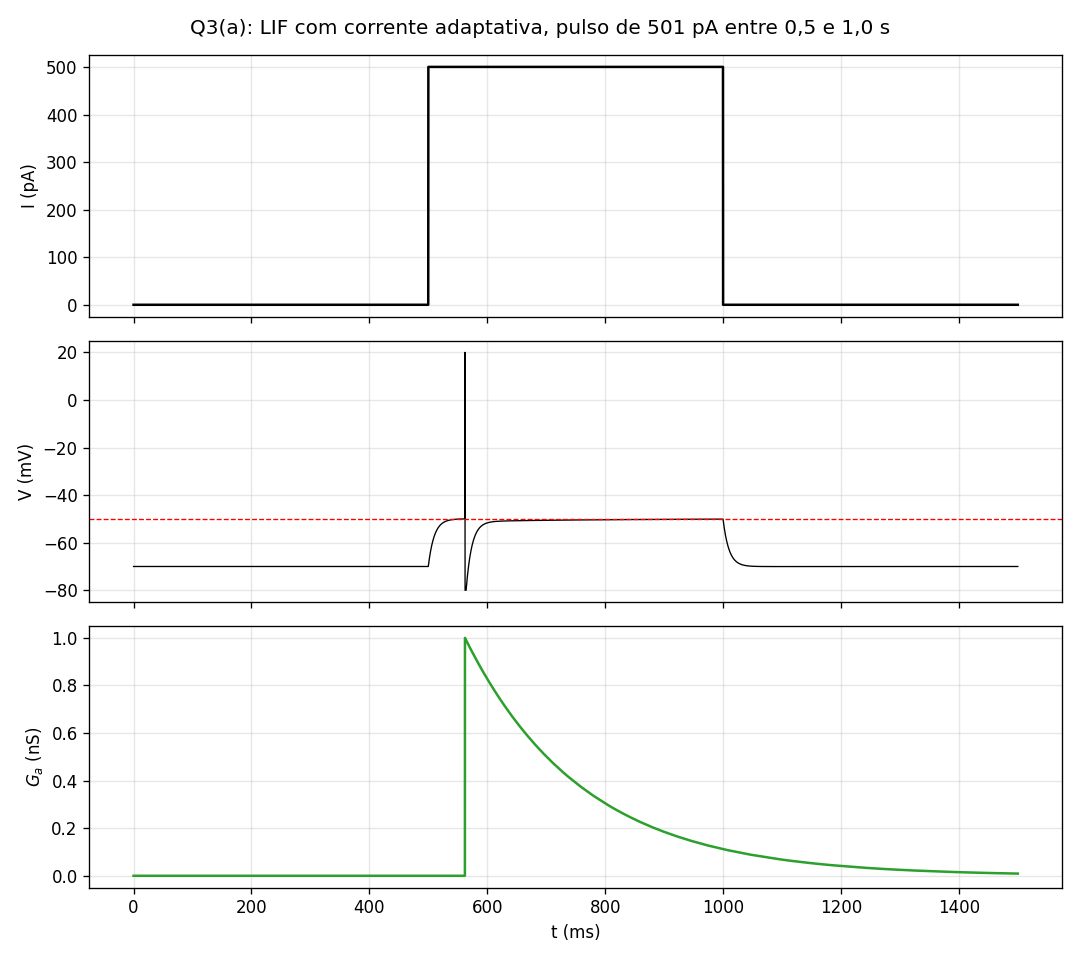
\includegraphics[width=0.85\textwidth]{q3a_pulso_adaptacao.png}\caption{Applied current, membrane potential and adaptation conductance for a $501$ pA pulse between $0.5$ and $1.0$ s.}\label{fig:q3a}\end{figure}
Only \textbf{one spike} occurs, $62.13$ ms after the pulse onset, in agreement with the analytical latency $\tau_m\ln\frac{RI}{RI-20}=10\ln501=62.17$ ms (with $G_a=0$). Afterwards $G_a=1$ nS and decays with $\tau_a$. A new spike requires $V_\infty^{\rm eff}=\frac{G_LV_{\rm rep}+G_aV_{\rm redef}+I}{G_L+G_a}\ge V_L$ ($G_L=1/R=25$ nS), i.e.
\begin{equation}
G_a\le\frac{I-I_L}{V_L-V_{\rm redef}}=\frac{501-500}{30}=\frac1{30}\ \mathrm{nS}.
\end{equation}
This needs $t-t_1=\tau_a\ln30=680$ ms, longer than the $438$ ms left in the pulse (at the end of the pulse $G_a=e^{-438/200}=0.11$ nS), so the neuron stays silent; $G_a$ keeps decaying after the pulse.

\subsection{(b) $f_1$--$I$ and $f_\infty$--$I$ curves}
Simulations of $5$ s for $400\le I\le800$ pA ($20$ pA steps); $T_1=t_2-t_1$ and $T_\infty$ is the last ISI (after about $25\tau_a$), $f_1=1/T_1$, $f_\infty=1/T_\infty$.
\begin{figure}[H]\centering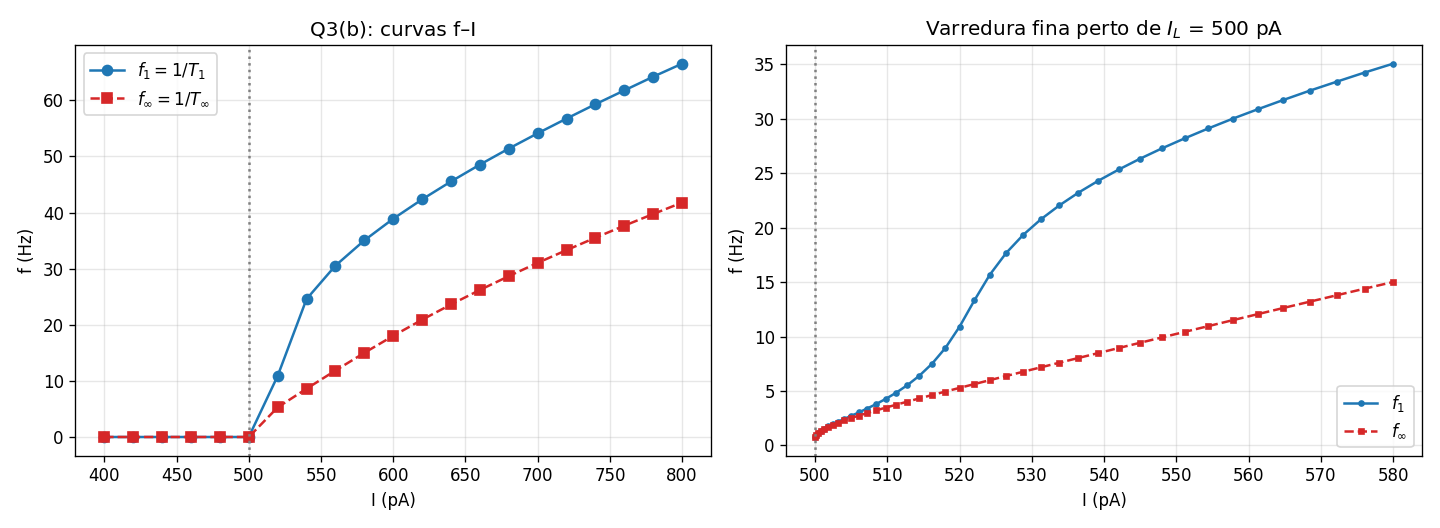
\includegraphics[width=\textwidth]{q3b_fI_adaptacao.png}\caption{Left: $f_1$ and $f_\infty$ vs.\ $I$. Right: fine sweep near $I_L=500$ pA.}\label{fig:q3b}\end{figure}
\begin{center}\begin{tabular}{cccccc}\toprule
$I$ (pA) & 500 & 520 & 600 & 700 & 800\\\midrule
$f_1$ (Hz) & 0 & 10.9 & 38.9 & 54.1 & 66.5\\
$f_\infty$ (Hz) & 0 & 5.3 & 18.0 & 31.0 & 41.8\\\bottomrule
\end{tabular}\end{center}
Adaptation lowers the steady rate, $f_\infty<f_1$ (about $60$--$65\%$ of $f_1$ at the highest currents). Both curves start at $I_L=500$ pA, where no spikes are produced (the response disappears with $I\le I_L$ even with $G_a=0$), and the fine sweep shows $f_1$ and $f_\infty$ decreasing continuously to $\approx0$ as $I\to I_L^+$ ($f\approx0.8$ Hz, i.e.\ $T\approx1.3$ s, already at $500.05$ pA and $f=0$ at $500.0$ pA; periods longer than the $5$ s window cannot be measured). The frequency therefore starts from zero: the model is \textbf{type I}, as the LIF neuron without adaptation (logarithmic divergence of the period at $I_L$).

\appendix
\section{Fortran code}
\subsection*{Common module}\lstinputlisting{../src/common/neuro_mod.f90}
\subsection*{Q1(a)}\lstinputlisting{../src/q1/q1a_fI_lif.f90}
\subsection*{Q2(a)}\lstinputlisting{../src/q2/q2a_fI_ruido.f90}
\subsection*{Q2(b)}\lstinputlisting{../src/q2/q2b_dt_rugosidade.f90}
\subsection*{Q2(c)}\lstinputlisting{../src/q2/q2c_cv_isi.f90}
\subsection*{Q3(a)}\lstinputlisting{../src/q3/q3a_pulso_adaptacao.f90}
\subsection*{Q3(b)}\lstinputlisting{../src/q3/q3b_fI_adaptacao.f90}
\end{document}
